\graphicspath{{quasidynamics/}}


\chapter{Convex Quasi-Dynamic Simulation of Rigid Point Clouds with Torsional Friction}
\label{sec:quasidynamics}

Many common manipulation tasks move slowly enough that velocities and Coriolis forces do not contribute meaningfully to the dynamics of the robot. As a result, quasi-dynamic simulation of these systems, in which all forces are assumed to be in equilibrium, can produce physically accurate results for use in motion-planning and control. Recent work has combined the quasi-dynamic model with a relaxed formulation of Coulomb friction, where the resulting dynamics are the solution to a convex quadratic program. We extend this recent work by directly manipulating rigid point clouds, without the need for meshing or decomposition into convex primitives. We also introduce a novel torsional friction model to mimic the frictional behaviors of the sorts of patch contacts that exist on real systems. These ideas are demonstrated in a grasping example, where a dense point cloud is manipulated with and without torsional friction, clearly showing the utility of the torsional friction model. 

The contents of this chapter have been previously published at the ICRA Leveraging Models in Contact-Rich Manipulation Workshop in \citet{tracy2023c}

\section{Introduction}


Accurate and computationally efficient simulation for contact-rich robotic manipulation tasks is crucial for developing model-based control policies. Existing simulators like Bullet \cite{coumans2015}, Drake \cite{tedrake2019a}, Dart \cite{lee2018}, and MuJoCo \cite{todorov2012a}, are able to model complex contact and friction interactions between a wide variety of geometries. While these simulators evaluate the full second-order dynamics of a robot, for many manipulation tasks, these second-order dynamics are not always necessary, and substantial computational savings are possible. 

For manipulation systems where objects are generally moving slowly, the velocities of the bodies are small enough that accelerations and Coriolis forces do not impact the dynamics in a meaningful way. As a result, quasi-dynamic \cite{mason2001} simulation methods, in which all forces are assumed to be in equilibrium, can be employed to solve for displacements in the configurations at each time step. 

This work is inspired by \cite{pang2018}, where a relaxed friction model from \cite{anitescu2006} is incorporated into a quasi-dynamic simulation method that treats actuators as impedances. Each simulation step consists of solving a small, well-defined convex Quadratic Program (QP), making the method fast and efficient, with virtually none of the stability problems encountered with full second-order dynamics formulations. This quasi-dynamic model was used successfully in a global planner in \cite{pang2023} where it was leveraged to build sophisticated motion plans for common manipulation tasks. In both of these works, only relatively simple shapes like spheres, capsules, and boxes were considered, due to the complications involved in collision checking.

In this paper, we make two contributions to the state of the art for quasi-dynamic simulation: the first is a computationally efficient framework for computing the dynamics of rigid objects whose complex geometry is represented by point clouds, and the second is a convex torsional friction model to effectively model patch contacts and avoid some of the non-physical behaviors seen when manipulating a rigid point cloud with rigid manipulators. Since the new torsional friction model is also represented as a convex constraint, each simulation step can still be computed efficiently by solving a QP. Together, these contributions enable fast and robust simulation of manipulation tasks involving complex non-convex geometries that would otherwise be challenging to decompose into simpler primitives.
% solver stuff 
%  \cite{mattingley2012} \cite{mehrotra1992} \cite{vandenberghe} \cite{nocedal2006a}
%  julia 
%  \cite{bezanson2017}
%  jax 
%  \cite{frostig2018, bradbury2018}
%  silico 
%  \cite{cleach2023a}
%  dojo 
%  \cite{howell2022}
%  Bullet \cite{coumans2015}, Drake \cite{tedrake2019a}, Dart \cite{lee2018}, and MuJoCo \cite{todorov2012a}.
% tao peng's stuff 
% first quasistatic \cite{pang2018}
% convex quasistatic \cite{pang2021}
% global planning \cite{pang2023} and gradients \cite{suh2020}
% differentiable optimization \cite{amos2019, agrawal2019, agrawal2019a}
% dcol \cite{tracy2022b}
% matt masons book 
% \cite{mason2001}
% anitescu \cite{anitescu2006}
% lcp sim \cite{stewart1996, stewart2000}
% \cite{boyd2004}
\section{Convex Quasi-Dynamic Models}

\begin{figure}[t]
\centering 
\begin{tikzpicture}
    \draw (0, 0) node[inner sep=0] {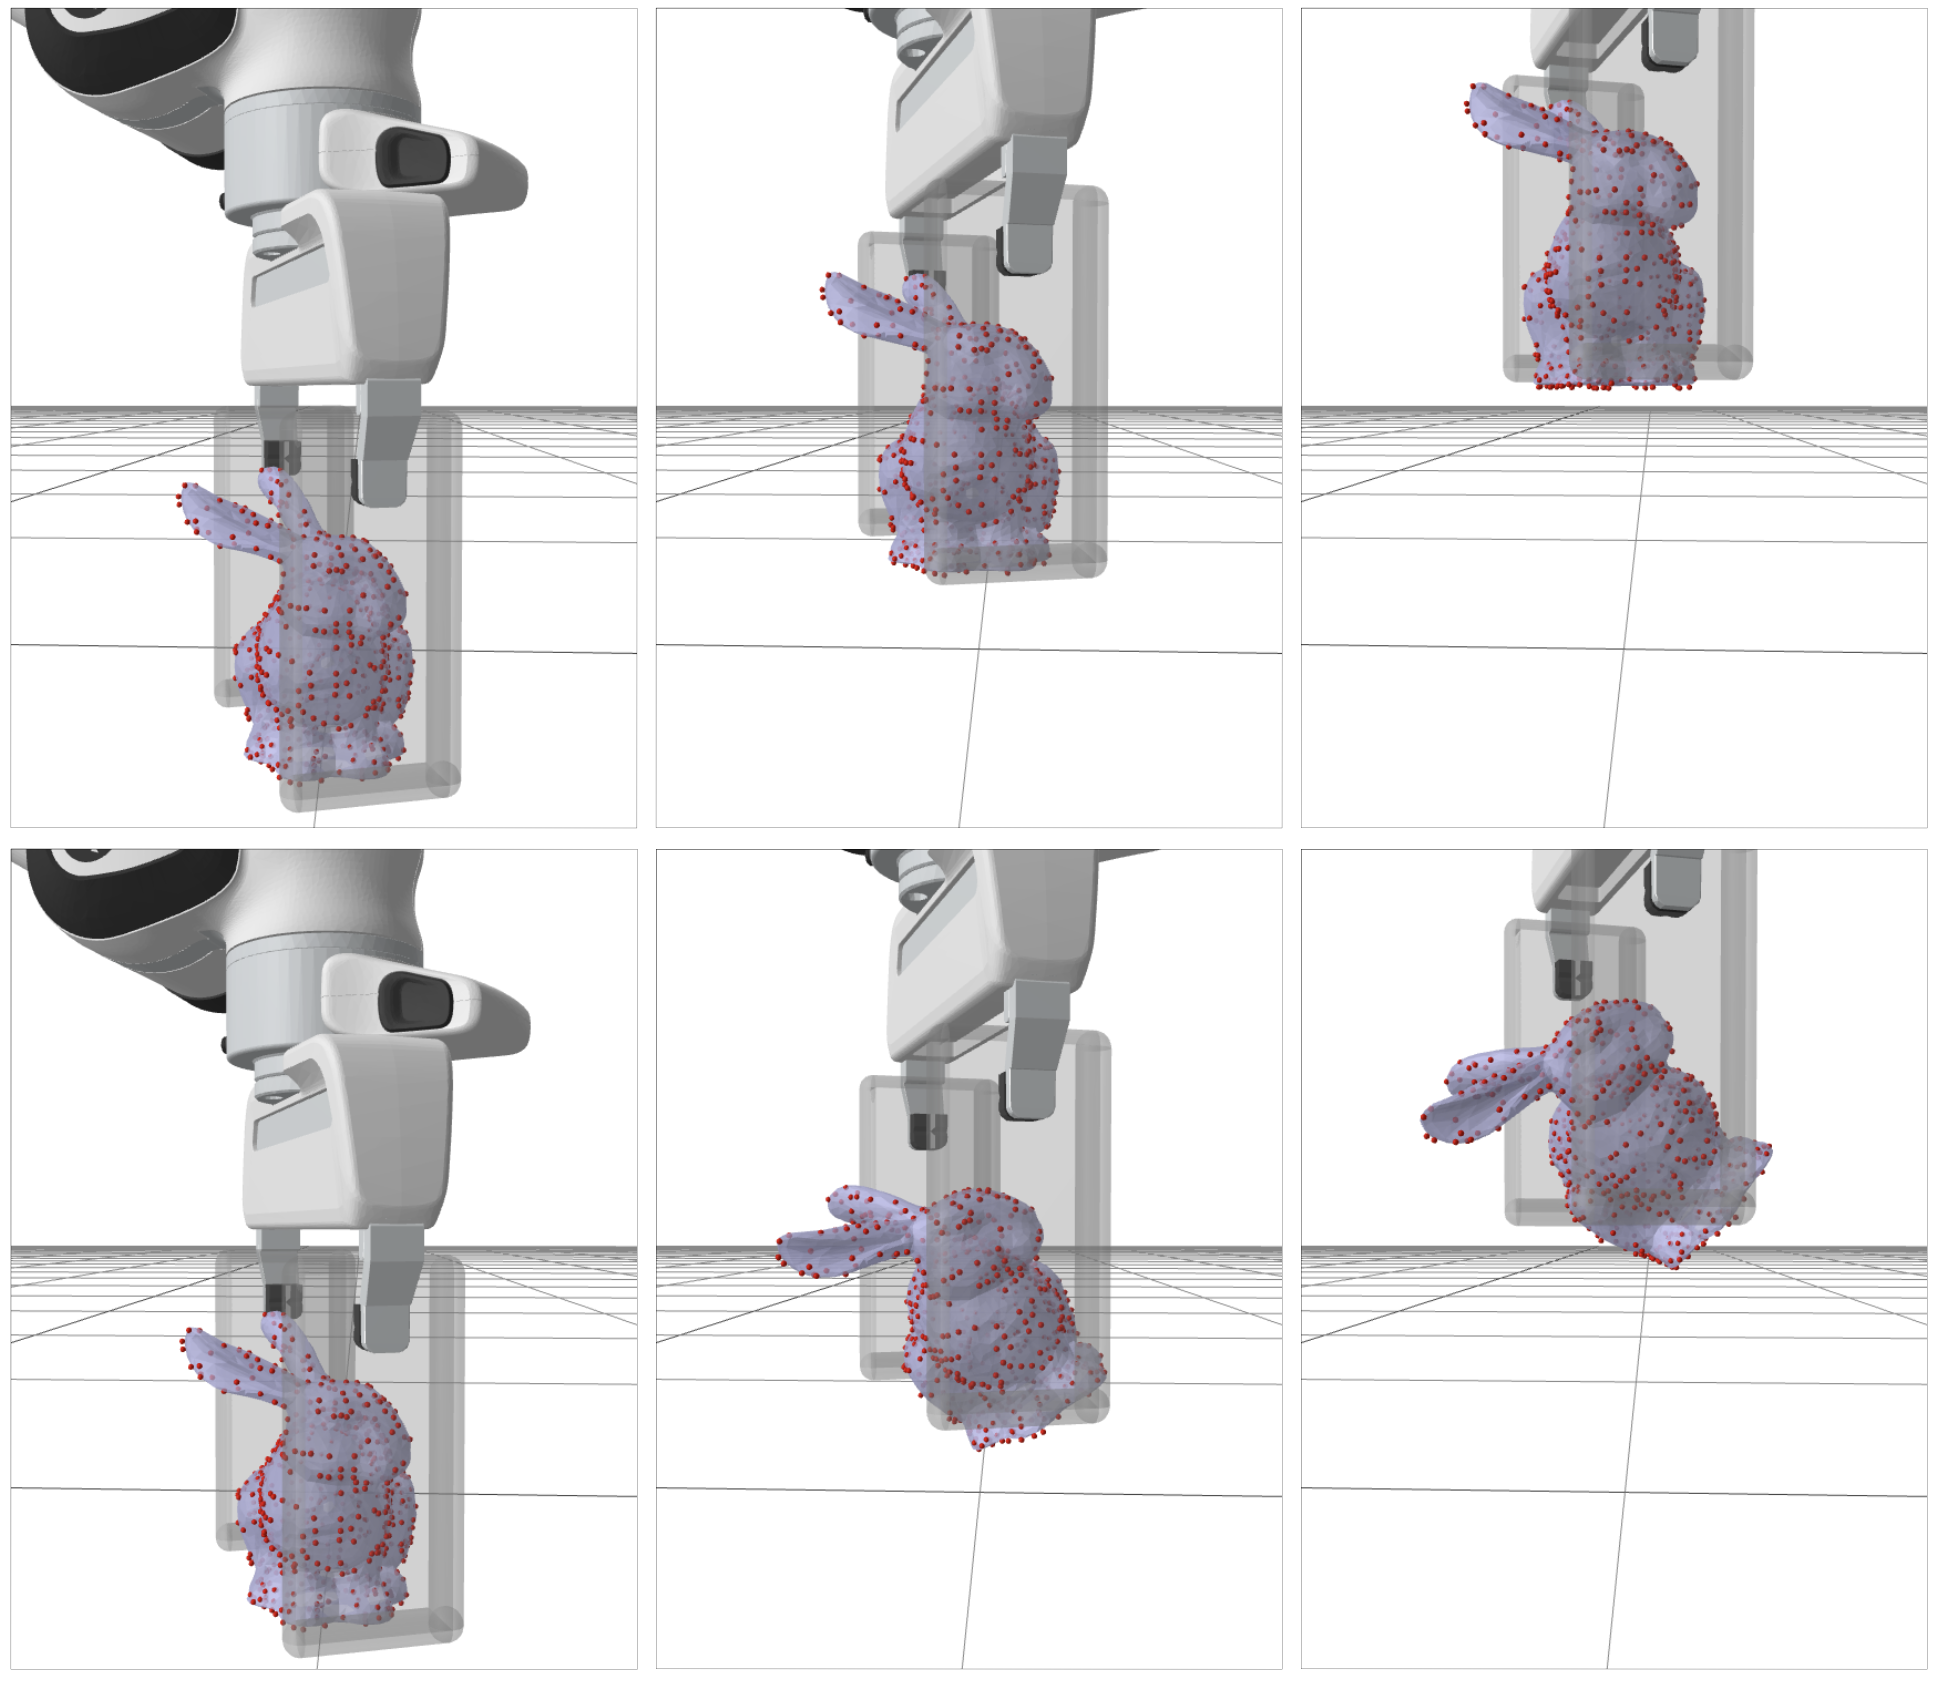
\includegraphics[width=4.3in]{figures/bunny_lift_3.png}};
    \draw (-4.6, -4.5) node {\small t = 0.0s};
    \draw (-1.0, -4.5) node {\small t = 0.7s};
    \draw (2.6, -4.5) node {\small t = 1.2s};
    % \draw (-3.2, 0) node {\color{white}{\Large Baseline}};
    \node at (-4.45,-.35) [fill=red!20, text=black] {Baseline};

    \node at (-4.75,4.35) [fill=green!20, text=black] {Ours};


    % \draw (-1.5, 6.5) node {\small no torsional frict.};
    % \draw (1.5, 6.5) node {\small with torsional frict.};
\end{tikzpicture}
\caption{Quasi-dynamic simulation of grasping a point cloud with and without torsional friction on the points. In the bottom sequence of frames, a simulation without torsional friction results in non-physical rotation of the bunny about single-point contacts with each gripper. Our method (top) includes torsional Coulomb friction at each contact point to avoid this behavior. %These constraints are formulated as linear inequalities and the simulation step is the solution to a convex quadratic program.
}
\label{fig:bunny_drop2}
\end{figure}


This section describes the general quasi-dynamic formulation with actuators modeled by impedances, closely following \cite{pang2018,pang2021}. The configuration of the whole system, $q \in \R{n_u + n_a}$, can be partitioned into an actuated part, $q_a \in \R{n_a}$, and an un-actuated part $q_u \in \R{n_u}$, stacked as $q = [q_a^T, q_u^T]^T$. In a quasi-dynamic model, there is no accumulation of velocity between time steps. As a result, a new velocity or a configuration displacement is computed at each time step. 
% When dealing with quaternions in the configurations, $\dot{q} \neq v$, but instead there exists a mapping between the two as $\dot{q} = G(q) v$. More details on this can be found in \cite{pang2018, mason2001}.  

The actuated degrees of freedom are treated as if they were controlled with impedance control. This means that we have some diagonal joint stiffness matrix $K_q \in \mathbb{S}^{n_a \times n_a}$, with the generalized force $\tau_k$ modeled as:
\begin{align}
    K_q \delta \bar{q}_a &= \tau_k,
\end{align}
where $\delta \bar{q}_a$ is the desired change in actuated configuration. The un-actuated degrees of freedom are simply acted upon by an external generalized force $\tau_a$, and contact forces.


\begin{figure}
\centering
\tdplotsetmaincoords{70}{110} % Set the viewing angle

\begin{tikzpicture}[scale=1.7,tdplot_main_coords]
    % Draw the axes
    \draw[thick,->] (0,0,0) -- (1,0,0) node[anchor=north east]{$x$};
    \draw[thick,->] (0,0,0) -- (0,1,0) node[anchor=north west]{$y$};
    \draw[thick,->] (0,0,0) -- (0,0,1) node[anchor=south]{$z$};
    % Draw the second sphere
    \tdplotsetrotatedcoords{0}{30}{0} % Set rotation for the second sphere
    \begin{scope}[tdplot_rotated_coords]
        \shade[ball color=blue!30, opacity=0.8] (0.6,2.2,3) circle (0.6);
        \shade[ball color=red!30, opacity=0.8] (1.0,0.8,5) circle (0.5);
        \begin{scope}[->, thick, black]
            \draw (0.68,1.917,3.404) -- ++(0.16,-.56,0.81) node[above]{$n$};
            \draw (0.68,1.917,3.404) -- ++(.07,0.82,0.56) node[above]{$d_1$};
            \draw (0.68,1.917,3.404) -- ++(-.98,-0.03,.17) node[right]{$d_2$};
        \end{scope}
    \end{scope}

           \shadedraw[tdplot_screen_coords,ball color = black] (1.03,1.5) circle (0.05) node[below,xshift=0.3cm]{$\alpha$};

           \shadedraw[tdplot_screen_coords,ball color = black] (-.2,2.3) circle (0.05) node[above,xshift=-0.3cm]{$\beta$};

           \coordinate (A_screen) at (0.0,1.10,1.735);
        \coordinate (B_screen) at (0., -.2,2.43);
        % \draw[dashed] (A_screen) -- (B_screen);
\draw[thick,decoration={brace,raise=4.5pt},decorate] (A_screen) -- (B_screen)
node[midway,below=4mm, left=.1mm]{$\phi$};

\end{tikzpicture}
\caption{Description of contact geometry for a given signed distance function $\phi = \|\beta - \alpha\|$, where $\alpha$ and $\beta$ are the closest points between two convex shapes. The unit contact normal vector $n$ extends from $\alpha$ to $\beta$, with a set of orthogonal tangent-plane vectors $d_1$ and $d_2$.}
\label{fig:contact_frame}
\end{figure}



\subsection{Contact and Friction Model}
Rigid contact and Coulomb friction can be incorporated into a quasi-dynamic model in the same fashion as a second-order dynamic model. First, collision information between pairs of convex objects can be computed with any number of methods, given that they return the closest points between objects as well as a contact normal vector \cite{gilbert1988,snethen2008,pan2012,tracy2022b}.
As shown in figure \ref{fig:contact_frame}, these closest points are denoted $\alpha$ and $\beta$, with the signed-distance function (SDF) between these denoted by $\phi$. Each of the $n_c$ pairwise contact interactions has its own $\alpha$, $\beta$, normal vector pointing from $\alpha$ to $\beta$, and a set of orthogonal tangent vectors $d_1$ and $d_2$. Together, the set $\{d_1, d_2, n\}$ describe a dextral triad of orthonormal vectors \cite{mitiguy2018, kane1983}. 

In \cite{anitescu2006}, Anitescu introduces a convex relaxation of tangential Coulomb friction that is exact when objects are sticking, and only introduces a slight "boundary layer" when objects are sliding. This relaxation allows for the inclusion of friction as a linear inequality in a quadratic program, enabling convex time-stepping methods \cite{pang2021}. In this work, we extend Anitescu's friction model to handle torsional friction about the contact normal.   This section omits indices that specify which contact pair is being considered for clarity, but the method extends to an arbitrary number of contacts.  

A Jacobian mapping forces $\lambda_i \in \R{3}$ at the contact point into generalized coordinates is calculated by taking the Jacobian of the following function with respect to the generalized velocity $v \in \R{n_v}$:
\begin{align}
    f(q,v) = \begin{bmatrix} \nu_\beta - \nu_\alpha \\ n^T(\omega_\beta -  \omega_\alpha) \end{bmatrix}, \label{eq:f}
\end{align}
where the relative velocity of the contact points is calculated by taking the difference between the velocity of $\beta$ ($\nu_\beta \in \R{3}$) and $\alpha$ ($\nu_\alpha \in \R{3}$). This Jacobian will be referred to as $J$:
\begin{align}
    J = \frac{\partial f(q,v)}{\partial v}.
\end{align}
where each vector in \eqref{eq:f} is resolved in the world frame. With this Jacobian, we can now write our friction constraints for a given point as the following:
\begin{align}
    \phi + [J^T(\tilde{n} + \tilde{d}_i)]^T  \delta q \geq 0 \quad \forall i
\end{align}
where $\tilde{n} = [n^T,0]^T$, and the the first four $\tilde{d}$'s describing the standard pyramidal tangential friction-cone approximation are the following:
\begin{align}
    \tilde{d}_1 &= \begin{bmatrix} \mu_v d_1 \\ 0 \end{bmatrix}, & \tilde{d}_2 &= \begin{bmatrix} \mu_v d_2 \\ 0 \end{bmatrix}, \\ \tilde{d}_3 &= \begin{bmatrix} -\mu_v d_1 \\ 0 \end{bmatrix},  & \tilde{d}_4 &= \begin{bmatrix} -\mu_v d_2 \\ 0 \end{bmatrix} .
\end{align}
We also introduce two more $\tilde{d}$'s describing torsional friction:
\begin{align}
    \tilde{d}_5 &= \begin{bmatrix} 0_3 \\ \mu_\omega \end{bmatrix}, & \tilde{d}_6 &= \begin{bmatrix} 0_3 \\ -\mu_\omega \end{bmatrix} ,
\end{align}
where $\mu_v \in \R{}_+$ is the tangential coefficient of friction and $\mu_\omega \in \R{}_+$ is the torsional coefficient of friction. These six linear inequalities describe the contact and friction for a given pair and can be vertically concatenated into a single $A\delta q \geq b$ constraint for convenience:
\begin{align}
    A &= \begin{bmatrix} J^T(\tilde{n} + \tilde{d}_1) \\ J^T(\tilde{n} + \tilde{d}_1) \\ \vdots \\ J^T(\tilde{n} + \tilde{d}_6) \end{bmatrix}, & b &= -\phi 1_6. \label{eq:a_b}
\end{align}
\subsection{Optimization Formulation}
The force balance for the actuated and un-actuated components of the configuration with contact forces can be posed as,
\begin{align}
    \begin{bmatrix} hK_q \delta q_a - hK_q\delta \bar{q}_a + \tau_a \\ \frac{1}{h}M_u\delta q_u - h \tau_u \end{bmatrix} + \sum_{n}^{n_c} A_j^T \lambda_j &= 0 ,\label{eq:stationarity}
\end{align}
where the contact/friction model is described as follows:
\begin{align}
    A_j \delta q &\geq b_j, \label{eq:pfeas}\\ 
    \lambda_j &\geq 0, \label{eq:dfeas} \\ 
    (A_j \delta q - b_j) \circ \lambda &= 0. \label{eq:compl}
\end{align}
These conditions are the KKT optimality conditions for a convex Quadratic Program (QP) where \eqref{eq:stationarity} is stationarity, \eqref{eq:pfeas} is primal feasibility, \eqref{eq:dfeas} is dual feasibility, and \eqref{eq:compl} is complementarity \cite{boyd2004}.  This QP is as follows:
 \begin{mini}|s|
{\delta q}{ \frac{1}{2}\delta q^T \begin{bmatrix} hK_q & 0 \\ 0 & M_u/h\end{bmatrix} \delta q - h\begin{bmatrix} K_q\delta \bar{q}_a + \tau_a \\ \tau_u \end{bmatrix}^T \delta q}{\label{opt}}{}
\addConstraint{A_j \delta q \geq}{b_j,}{ \quad \quad \forall j \in \mathcal{E}}
\end{mini}
where $\mathcal{E}$ is the set of contact pairs being considered and $h \in \R{}_+$ is the time-step size.  For large point clouds, this pruning of constraints is critical for keeping the resulting QP small. %For QP's of this size, a primal-dual interior-point method can reliably solve these to low tolerance with low
Another benefit to the QP formulation is differentiability: In recent years, differentiable convex optimization has enabled smooth automatic differentiation through QP solvers with good results \cite{tracy2022a, howell2022, amos2019,suh2020}.
\section{Numerical Examples}
Two examples are shown to demonstrate the behavior and utility of our formulation: The first example is a simple spinning sphere that showcases the tightness of the relaxed friction constraints, and the second is a more practical example of gripping a dense point cloud with and without torsional friction. 
\subsection{Torsional Boundary Layer}
\begin{figure}
    \centering
    \includegraphics[width=.55\textwidth]{figures/torsion_slipping.tikz}
    \caption{Visualization of the boundary layer that exists only when a point in contact begins rotating due to an external torque $\tau$. In the exact same fashion as the tangential friction constraints, a boundary layer is introduced during sliding that is proportional to the time step $h$.}
    \label{fig:boundary_layer}
\end{figure}
To demonstrate the boundary layer induced by the relaxed torsional friction constraints, figure \ref{fig:boundary_layer} demonstrates what happens when a sphere in contact with the floor is spun. An increasing external torque is applied to the sphere, and up until the maximum allowable friction torque is saturated, the sphere does not move. Once the external torque exceeds this limit, the sphere begins to spin and lifts off from the surface by a fraction of a centimeter. 

This boundary-layer behavior mirrors the tangential friction case, where this is the only deviation from Coulomb friction and the size of this boundary layer decreases with step size. For most manipulation tasks that aren't pushing or sliding, full sticking behavior is desirable, making this relaxed model appropriate. 

\subsection{Grasping a Point Cloud}
In this example, shown in Fig. \ref{fig:bunny_drop2}, parallel grippers are used to grasp a point-cloud bunny with and without torsional friction. The bunny was modeled as a rigid body with 992 points, each of which was constrained to consider the floor, the left gripper, and the right gripper. The simulator checks the signed distance function for each of these 992 points with respect to the three objects, and selects five points for each object to include in the quadratic program. Each of the selected points contributes the constraints shown in \eqref{eq:a_b} to the optimization. 

While these five closest points in question can change from time step to time step, the size of the QP remains the same. 
The resulting QP for this example has 13 primal variables with 80 inequality constraints, and is solved with a custom primal-dual interior-point algorithm \cite{mehrotra1992, nocedal2006, vandenberghe} that leverages templating based on the number of contacts considered during a simulation. 

When the grippers close on the bunny, it is possible for there to be single points of contact with each gripper. In this case, the lack of torsional friction results in the bunny rotating about these contact points. While this is technically correct behavior given point contacts, the true system does not exhibit this behavior due to patch-contact effects, resulting in a significant sim-to-real gap. On a real robotic system, there is always some compliance either on the gripper or the object that manifests in a patch contact instead of a point contact. The patch contact provides a lever arm for torsional friction, preventing the bunny from pivoting.  Just like with tangential friction, the torsional friction is proportional to the normal force on the contact.

\emph{By including torsional friction for each point contact, we are able to replicate torsional friction behaviors while still treating the object as a rigid point cloud.}


The full simulation step takes less than 90 $\mu s$ for a time step size of $h = 0.01 s$., with the profile of this function shown in Fig. \ref{fig:speeds}.\footnote{Timing results are reflective of a Mac M1 Pro, running Julia 1.9.2} Since a majority of the time is spent solving the QP, there is reason to believe this sort of simulation makes more sense on a CPU than a GPU, despite the possibility of a very dense point cloud. There may be cases where the point cloud is dense enough that computing and sorting all of the pairwise contacts is the limiting computational factor, in which case a GPU implementation would make more sense. 
\begin{figure}
\centering 
\begin{tikzpicture}[scale=0.70]
   \pie[rotate=0, text=pin,color={blue!10, red!10, orange!10, blue!30}]  
 {11/SDFs,  16.6/sort, 8/build QP, 64.3/solve QP}  
\end{tikzpicture}  
\caption{Average timing results for a step in the quasi-dynamic simulator with the bunny where the total time was $<$90 $\mu s$  for a time step size of $h = 0.01s$. A majority of the time is spent solving the QP, despite the fact there are almost 3,000 signed distance functions evaluations. %The QP minimizes a function with respect to 13 variables subject to 80 inequalities.
}
\label{fig:speeds}
\end{figure}

%%% Local Variables:
%%% coding: utf-8
%%% mode: latex
%%% TeX-engine: xetex
%%% TeX-master: "../thesis"
%%% End: